\documentclass{beamer}

\mode<presentation> {
\usetheme{Montpellier}
}

\usepackage{graphicx}
\usepackage{booktabs}
\usepackage[utf8]{inputenc}
\setcounter{tocdepth}{2}
\graphicspath{{Figures/}}

\title[Neural Networks]{Technical introduction to Neural Networks}
%\author{Nicolas Le Hir} % Your name
\date{\today}

\begin{document}

\begin{frame}
\titlepage 
\end{frame}

\begin{frame}
    \tableofcontents
\end{frame}

\section{Vectors, matrices, neural nets}%
\label{sec:vectors_matrices_neural_nets}

\begin{frame}
\frametitle{Elementary neuron}
    A \textbf{{neuron}} is a \textbf{{mapping}} from a multidimensional input
    $x=(x_1,...,x_n)$ to a real number $y$.\end{frame}
\begin{frame}

\frametitle{Elementary neuron}
    A \textbf{{neuron}} is a \textbf{{mapping}} from a multidimensional input
    $x=(x_1,...,x_n)$ to a real number $y$. In it's simplest form, this
    function depends on \textbf{{parameters}} called \textbf{{weights}}
    $w=(w_1,...,w_n)$.  We can see it as a function $ f : x
    \rightarrow y$ with :
    \begin{equation}
        y=\sigma( \sum^{n}_{i=1} x_iw_i )
    \end{equation}
\end{frame}


\begin{frame}
\frametitle{Elementary neuron}
    A \textbf{{neuron}} is a \textbf{{mapping}} from a multidimensional input
    $x=(x_1,...,x_n)$ to a real number $y$. In it's simplest form, this
    function depends on \textbf{{parameters}} called \textbf{{weights}}
    $w=(w_1,...,w_n)$.  We can see it as a function $ f : x
    \rightarrow y$ with :
    \begin{equation}
        y=\sigma( \sum^{n}_{i=1} x_iw_i )
    \end{equation}
Where $\sigma$ is a non linear function, for instance a \textbf{{sigmoid}}.
\end{frame}

\begin{frame}{Notation with vectors}
    The sum $   \sum^{n}_{i=1} x_iw_i  $ can also be written this way : 
    \begin{equation}
        xw^T
    \end{equation}
    This means a \textbf{{product}} of \textbf{{two matrices}} (a vector is
    also a matrix : it is just a matrix with only one line or only one column) : 
      : 
\end{frame}
\begin{frame}{Notation with vectors}
    The sum $   \sum^{n}_{i=1} x_iw_i  $ can also be written this way : 
    \begin{equation}
        xw^T
    \end{equation}
    This means a \textbf{{product}} of \textbf{{two matrices}} (a vector is
    also a matrix : it is just a matrix with only one line or only one column) : 
      : 
    \begin{itemize}
        \item $x=(x_1,...,x_n)$
                \item 
$$
w^T=
\begin{pmatrix}
w_1\\
w_2\\
\vdots\\
w_n
\end{pmatrix}
$$
    \end{itemize}
\end{frame}

\begin{frame}{Matrices}
    A matrix is an array used to store data. It has \textbf{{lines}}  and
    \textbf{{columns}} 
$$
A=
\begin{pmatrix}
1 & 4 & 1 \\
0 & 1 & 2 \\
0 & 0 & 1
\end{pmatrix}
$$
\end{frame}


\begin{frame}{Matrices}
    A matrix is an array used to store data. It has \textbf{{lines}}  and
    \textbf{{columns}} 
$$
A=
\begin{pmatrix}
1 & 4 & 1 \\
0 & 1 & 2 \\
0 & 0 & 1
\end{pmatrix}
$$
    $A_{ij}$ means the element at line $i$ and columns $j$.
\end{frame}

\begin{frame}{Matrices}
    A matrix is an array used to store data. It has \textbf{{lines}}  and
    \textbf{{columns}} 
$$
A=
\begin{pmatrix}
1 & 4 & 1 \\
0 & 1 & 2 \\
0 & 0 & 1
\end{pmatrix}
$$
    $A_{ij}$ means the element at line $i$ and columns $j$.
    \begin{itemize}
        \item $A_{12}=\;$?
        \item $A_{31}=\;$?
        \item $A_{33}=\;$?
    \end{itemize}
\end{frame}

\begin{frame}{Matrices}
    A matrix is an array used to store data. It has \textbf{{lines}}  and
    \textbf{{columns}} 
$$
A=
\begin{pmatrix}
1 & 4 & 1 \\
0 & 1 & 2 \\
0 & 0 & 1
\end{pmatrix}
$$
    $A_{ij}$ means the element at line $i$ and columns $j$.
    \begin{itemize}
        \item $A_{12}=4$
        \item $A_{31}=0$
        \item $A_{33}=1$
    \end{itemize}
\end{frame}

\begin{frame}{Product of matrices}
    \begin{itemize}
        \item If matrix $A$ has $p$ columns and matrix $B$ has $p$ lines, we
            can compute the product of the two $AB$ of the two matrices in the
            following way : 
            \begin{equation}
                AB_{ij}= \sum^{n}_{k=1} A_{ik}B_{kj}
            \end{equation}
    \end{itemize}
\end{frame}

\begin{frame}{Product of matrices}
    \begin{itemize}
        \item If matrix $A$ has $p$ columns and matrix $B$ has $p$ lines, we
            can compute the product of the two $AB$ of the two matrices in the
            following way : 
            \begin{equation}
                AB_{ij}= \sum^{n}_{k=1} A_{ik}B_{kj}
            \end{equation}
        \item This kind of computation is very often used
    \end{itemize}
\end{frame}

\begin{frame}{Product of matrices}
    \begin{itemize}
        \item If matrix $A$ has $p$ columns and matrix $B$ has $p$ lines, we
            can compute the product of the two $AB$ of the two matrices in the
            following way : 
            \begin{equation}
                AB_{ij}= \sum^{n}_{k=1} A_{ik}B_{kj}
            \end{equation}
        \item This kind of computation is very often used
        \item It is way more convenient and concise to use
        \item We will use it when studying neural networks
    \end{itemize}
\end{frame}
%\begin{frame}{Examples}
%    \[ \left( \begin{array}{cc}
%1 & 0 \\
%0 & 1
%\end{array} \right)
%%
%\left( \begin{array}{cc}
%1 & 0 \\
%0 & 1
%\end{array} \right)
%\]
%\end{frame}

\begin{frame}{Examples}
   \[
\begin{pmatrix}
1 & 4 & 1 \\
0 & 1 & 2 \\
0 & 0 & 1
\end{pmatrix}
\begin{pmatrix}
0 & 0 & 0 \\
0 & 0 & 0 \\
0 & 0 & 0
\end{pmatrix}
    =\text{?} 
\] 
\end{frame}

\begin{frame}{Examples}
   \[
\begin{pmatrix}
1 & 4 & 1 \\
0 & 1 & 2 \\
0 & 0 & 1
\end{pmatrix}
\begin{pmatrix}
0 & 0 & 0 \\
0 & 0 & 0 \\
0 & 0 & 0
\end{pmatrix}
    =
\begin{pmatrix}
0 & 0 & 0 \\
0 & 0 & 0 \\
0 & 0 & 0
\end{pmatrix}
\] 
\end{frame}


\begin{frame}{Examples}
   \[
\begin{pmatrix}
1 & 4 & 1 \\
0 & 1 & 2 \\
0 & 0 & 1
\end{pmatrix}
\begin{pmatrix}
1 & 0 & 0 \\
0 & 1 & 0 \\
0 & 0 & 1
\end{pmatrix}
    =\text{?} 
\] 
\end{frame}

\begin{frame}{Examples}
   \[
\begin{pmatrix}
1 & 4 & 1 \\
0 & 1 & 2 \\
0 & 0 & 1
\end{pmatrix}
\begin{pmatrix}
1 & 0 & 0 \\
0 & 1 & 0 \\
0 & 0 & 1
\end{pmatrix}
    =
\begin{pmatrix}
1 & 4 & 1 \\
0 & 1 & 2 \\
0 & 0 & 1
\end{pmatrix}
\] 
\end{frame}



\begin{frame}{Examples}
   \[
\begin{pmatrix}
1 & 4 & 1 \\
0 & 1 & 2 \\
0 & 0 & 1
\end{pmatrix}
\begin{pmatrix}
1 & 0 & 0 \\
0 & 2 & 0 \\
1 & 0 & 0
\end{pmatrix}
    =\text{?} 
\] 
\end{frame}

\begin{frame}{Examples}
   \[
\begin{pmatrix}
1 & 4 & 1 \\
0 & 1 & 2 \\
0 & 0 & 1
\end{pmatrix}
\begin{pmatrix}
1 & 0 & 0 \\
0 & 2 & 0 \\
1 & 0 & 0
\end{pmatrix}
    =
\begin{pmatrix}
2 & 8 & 0 \\
2 & 2 & 0 \\
1 & 0 & 0
\end{pmatrix}
\] 
\end{frame}


\begin{frame}{Examples}
   \[A=
\begin{pmatrix}
1 & 1 & 1 \\
1 & 1 & 1 \\
1 & 1 & 1
\end{pmatrix}
\] 
What is $A^n$ ?
\end{frame}


\begin{frame}{Examples}
    \begin{itemize}
        \item $x=(x_1,...,x_n)$
        \item $w=(w_1,...,w_n)$
    \end{itemize}
    \begin{equation}
        xw^T=\text{?}
    \end{equation}
\end{frame}

\begin{frame}{Examples}
    \begin{itemize}
        \item $x=(x_1,...,x_n)$
        \item $w=(w_1,...,w_n)$
    \end{itemize}
    \begin{equation}
    xw^T= \sum^{n}_{i=1} x_iw_i
    \end{equation}
\end{frame}

\begin{frame}{Neural networks}
    \begin{itemize}
        \item $\sigma(xw^T )$ allows us to compute the output of a
            \textbf{{single neuron}} 
        \item But we will often have \textbf{{several neurons}} outputting a
            result.
        \item These neurons are organized in a network called neural network.
    \end{itemize}
\end{frame}

\begin{frame}{Neural networks}
    \begin{itemize}
        \item These neurons are organized in a network called neural network.
            \begin{figure}[htpb]
                \centering
                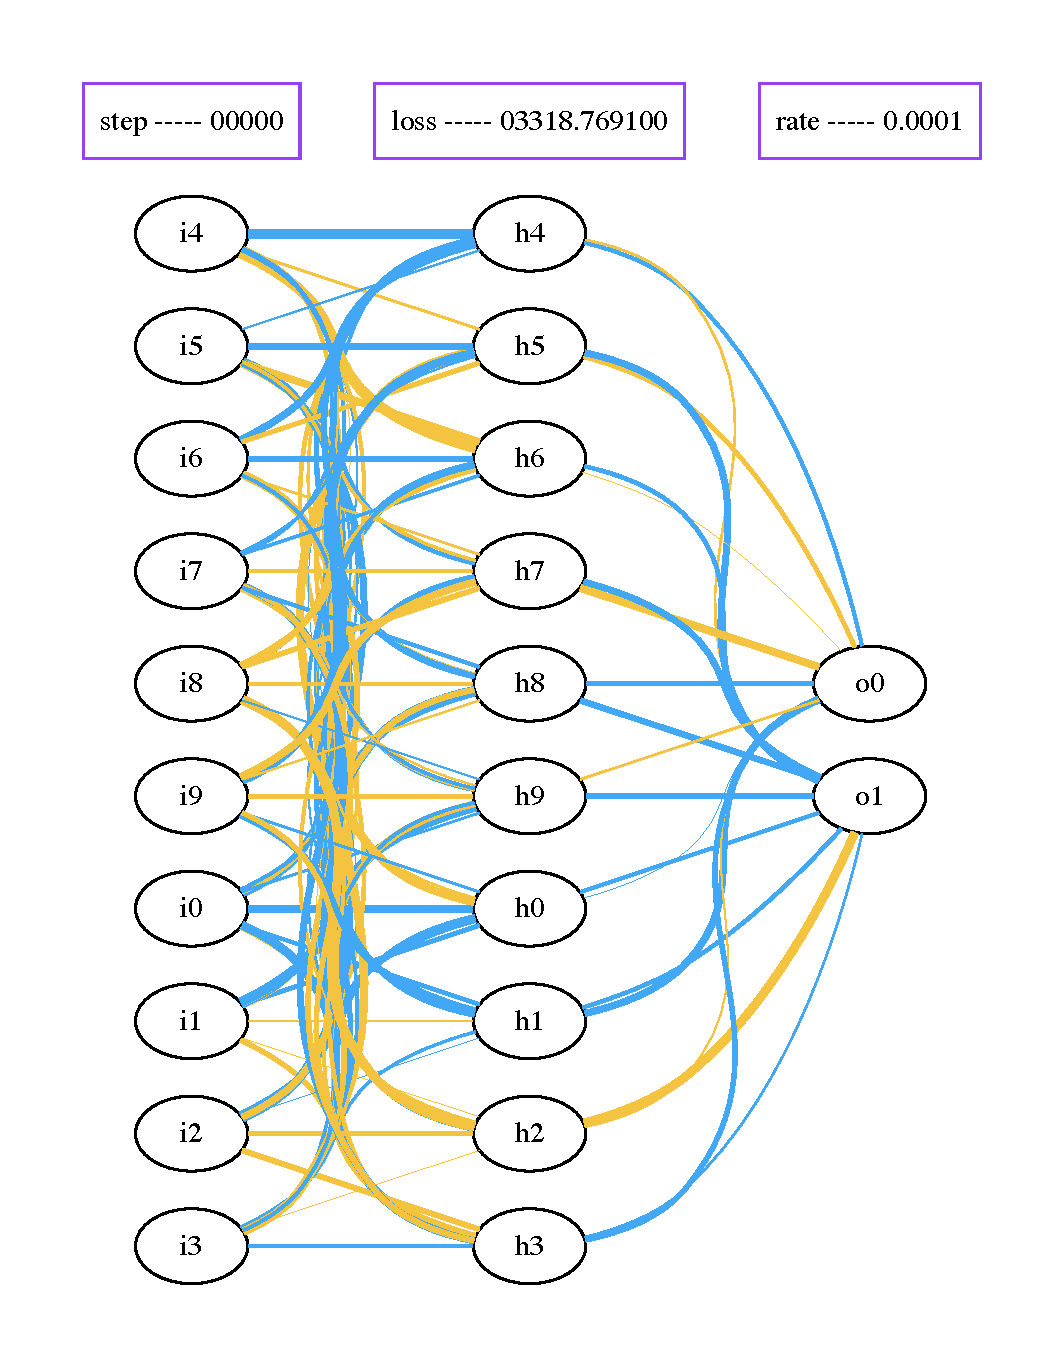
\includegraphics[width=0.5\linewidth]{net_0}
                \label{fig:name}
            \end{figure}
    \end{itemize}
\end{frame}

\begin{frame}{Matrices and networks}
    \begin{itemize}
        \item Let $W=[W_{ij}]$ be the matrices of weights between neuron $i$ of
            the left layer and neuron $j$ of the middle layer.
            \begin{figure}[htpb]
                \centering
                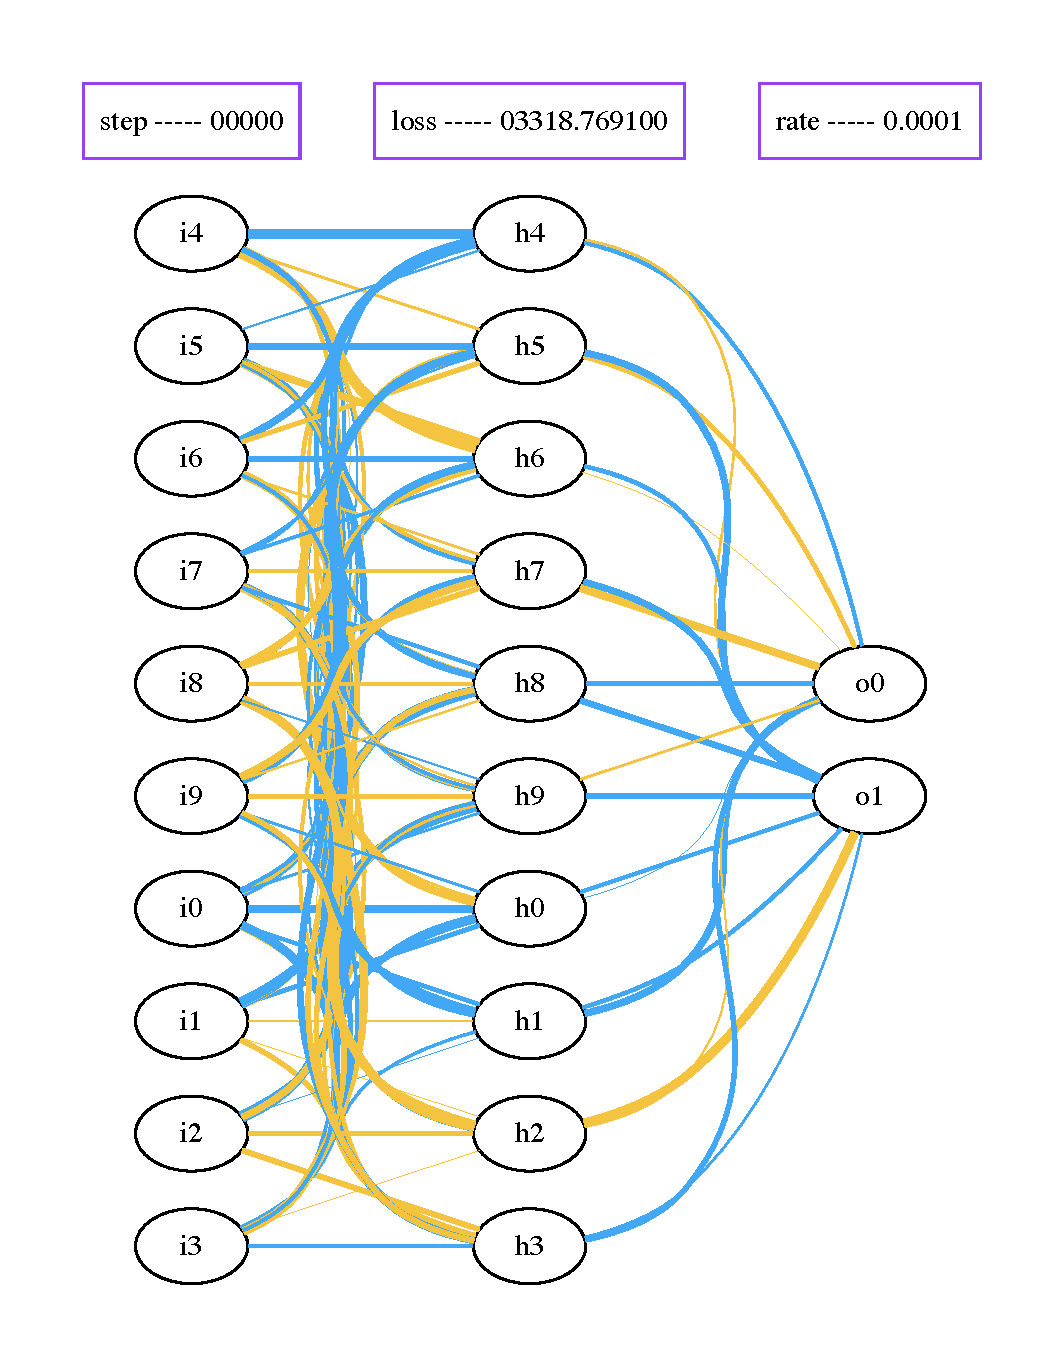
\includegraphics[width=0.5\linewidth]{net_0}
                \label{fig:name}
            \end{figure}
    \end{itemize}
\end{frame}


\begin{frame}{Matrices and networks}
    \begin{itemize}
        \item Let $W=[W_{ij}]$ be the matrices of weights between neuron $i$ of
            the left layer and neuron $j$ of the middle layer.
        \item How can we write the inputs $b_j$ of the middle layer as a
            function of the outpus $x_k$ of the left layer ?
            \begin{figure}[htpb]
                \centering
                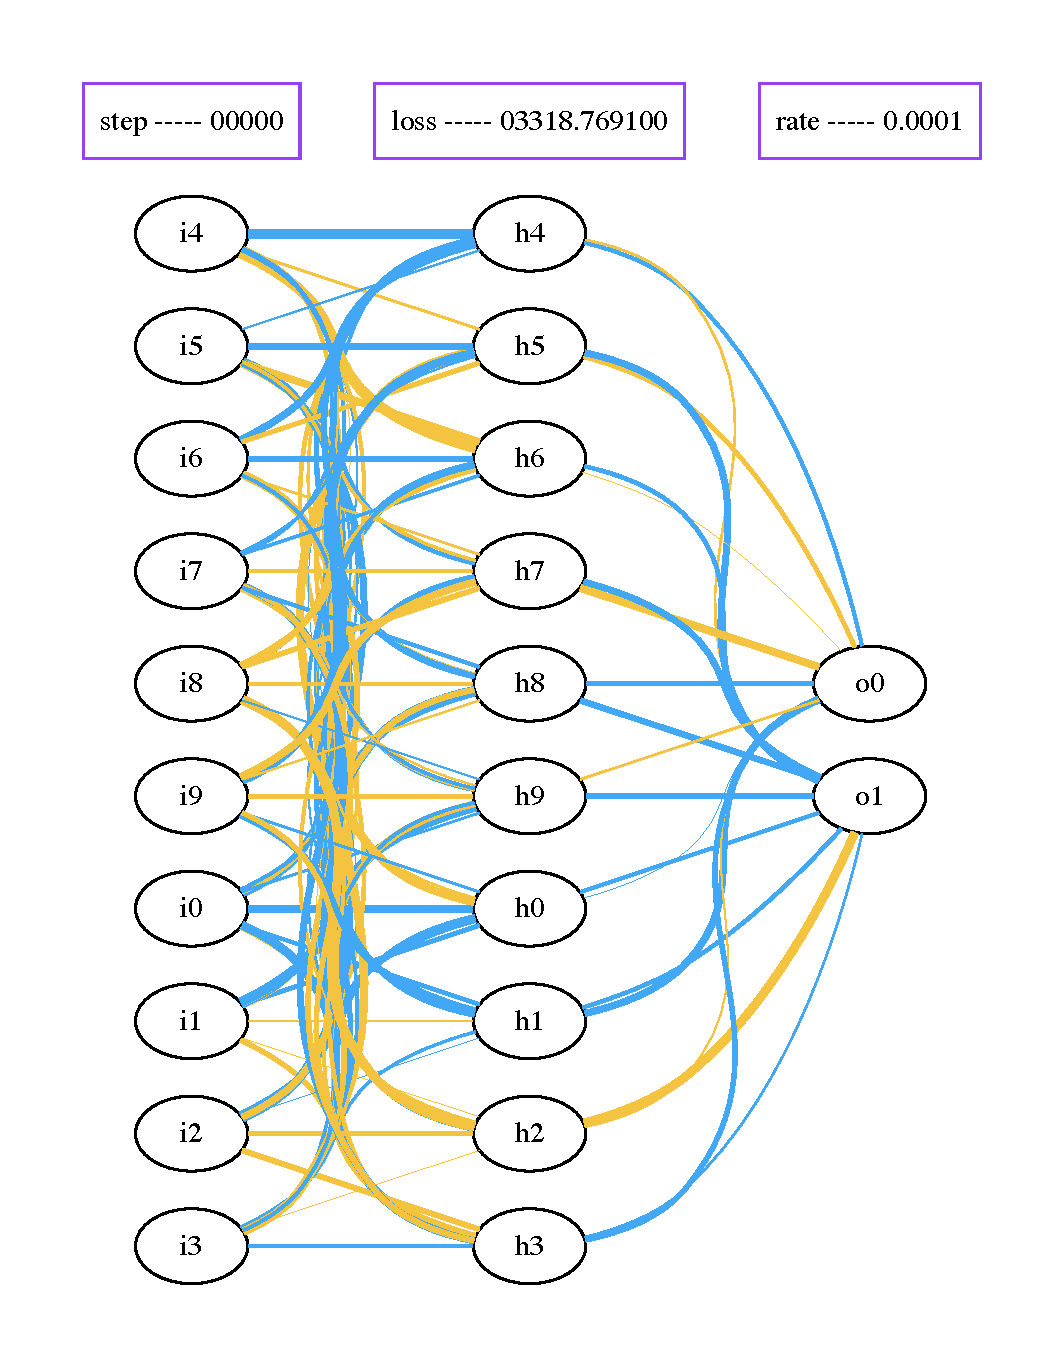
\includegraphics[width=0.4\linewidth]{net_0}
                \label{fig:name}
            \end{figure}
    \end{itemize}
\end{frame}

\begin{frame}{Matrices and networks}
    \begin{itemize}
        \item let $w=[w_{ij}]$ be the matrices of weights between neuron $i$ of
            the left layer and neuron $j$ of the middle layer.
        \item how can we write the inputs $b_j$ of the middle layer as a
            function of the outpus $x_k$ of the left layer ?
            \begin{equation}
                b_j= \sum^{n}_{k=1}x_kw_{kj} 
            \end{equation}
            \begin{figure}[htpb]
                \centering
                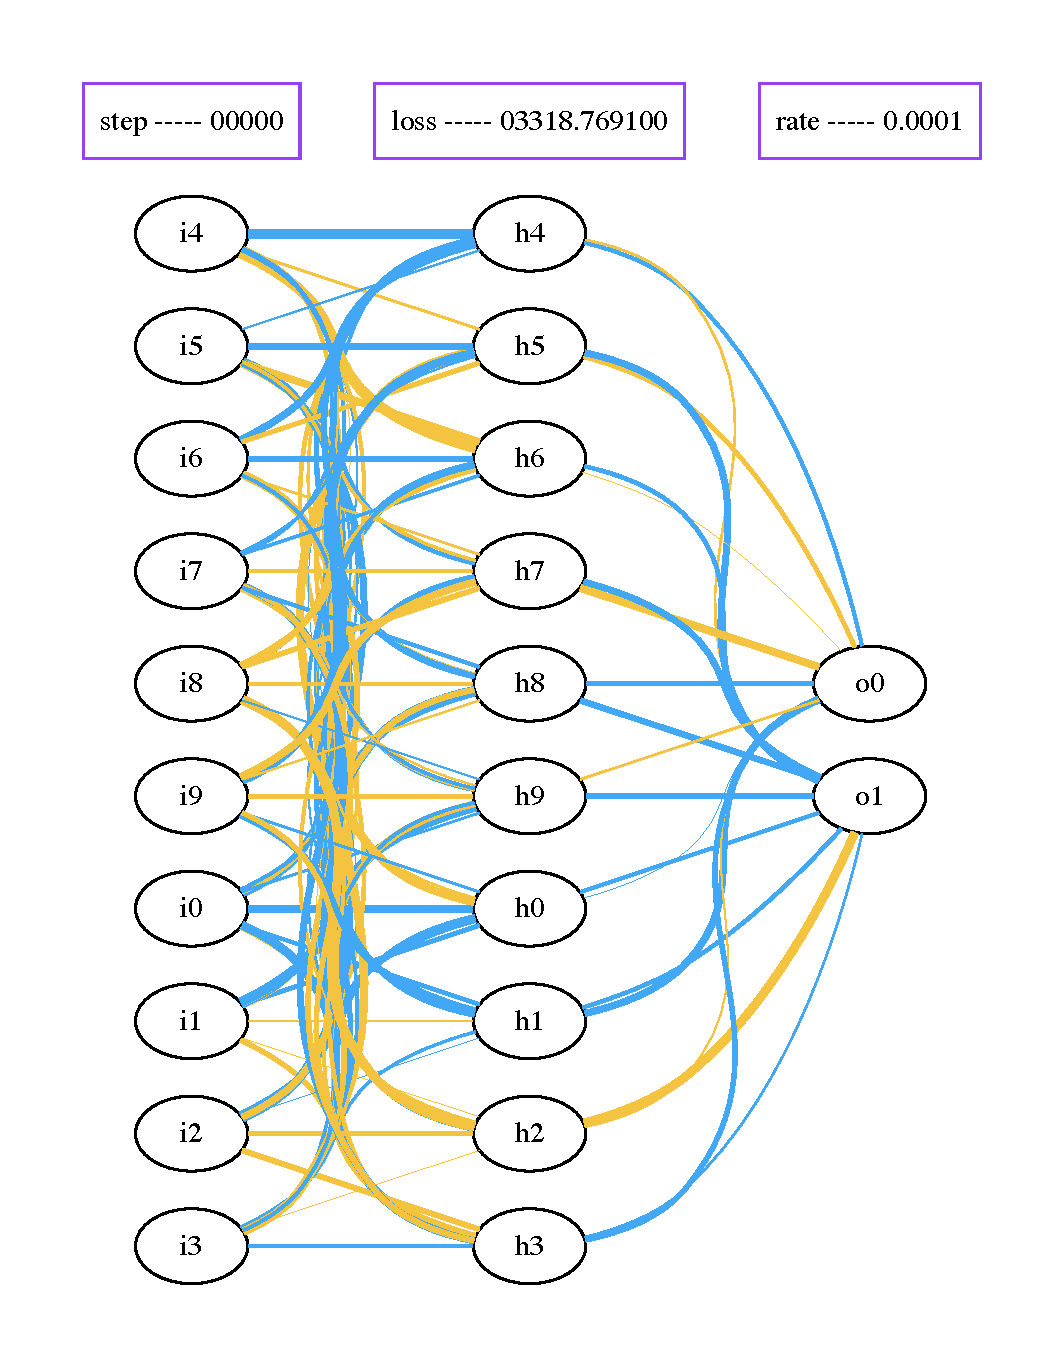
\includegraphics[width=0.3\linewidth]{net_0}
                \label{fig:name}
            \end{figure}
    \end{itemize}
\end{frame}

\begin{frame}{Matrices and networks}
    \begin{itemize}
        \item let $w=[w_{ij}]$ be the matrices of weights between neuron $i$ of
            the left layer and neuron $j$ of the middle layer.
            \begin{equation}
                b_j= \sum^{n}_{k=1}x_kw_{kj} 
            \end{equation}
        \item And in terms of matrices ? with : 
            \begin{itemize}
                \item $b=(b_1,...,b_n)$
                \item $x=(x_1,..,x_n)$
            \end{itemize}
            \begin{figure}[htpb]
                \centering
                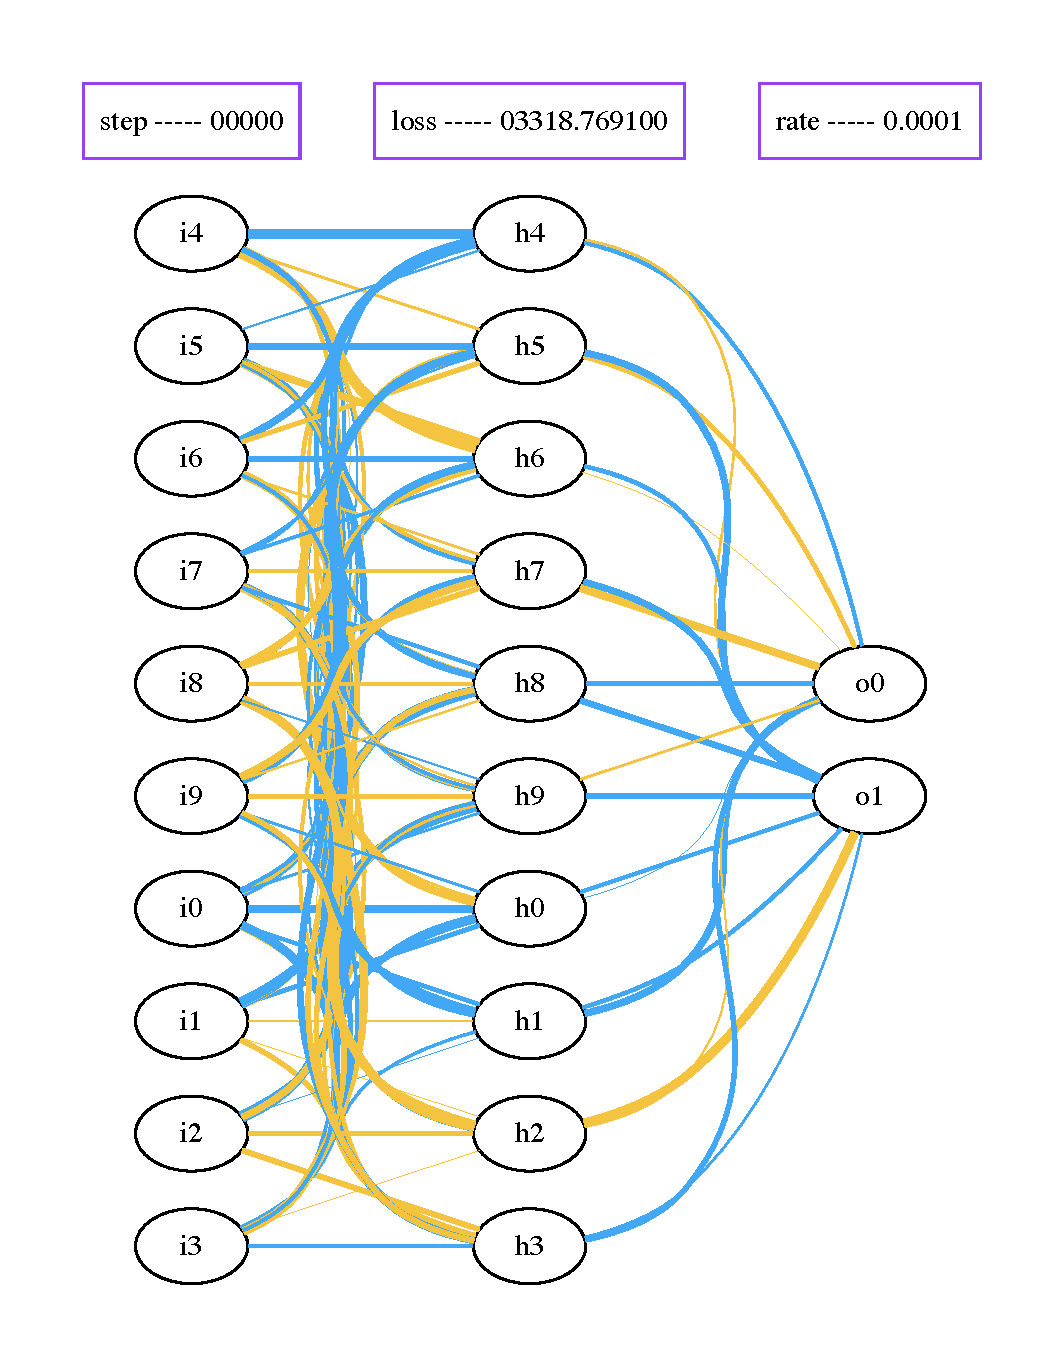
\includegraphics[width=0.2\linewidth]{net_0}
                \label{fig:name}
            \end{figure}
    \end{itemize}
\end{frame}


\begin{frame}{Matrices and networks}
    \begin{itemize}
        \item let $w=[w_{ij}]$ be the matrices of weights between neuron $i$ of
            the left layer and neuron $j$ of the middle layer.
            \begin{equation}
                b_j= \sum^{n}_{k=1}x_kw_{kj} 
            \end{equation}
        \item And in terms of matrices ? with : 
            \begin{itemize}
                \item $b=(b_1,...,b_n)$
                \item $x=(x_1,..,x_n)$
            \end{itemize}
            \begin{equation}
                b=xw
            \end{equation}
            \begin{figure}[htpb]
                \centering
                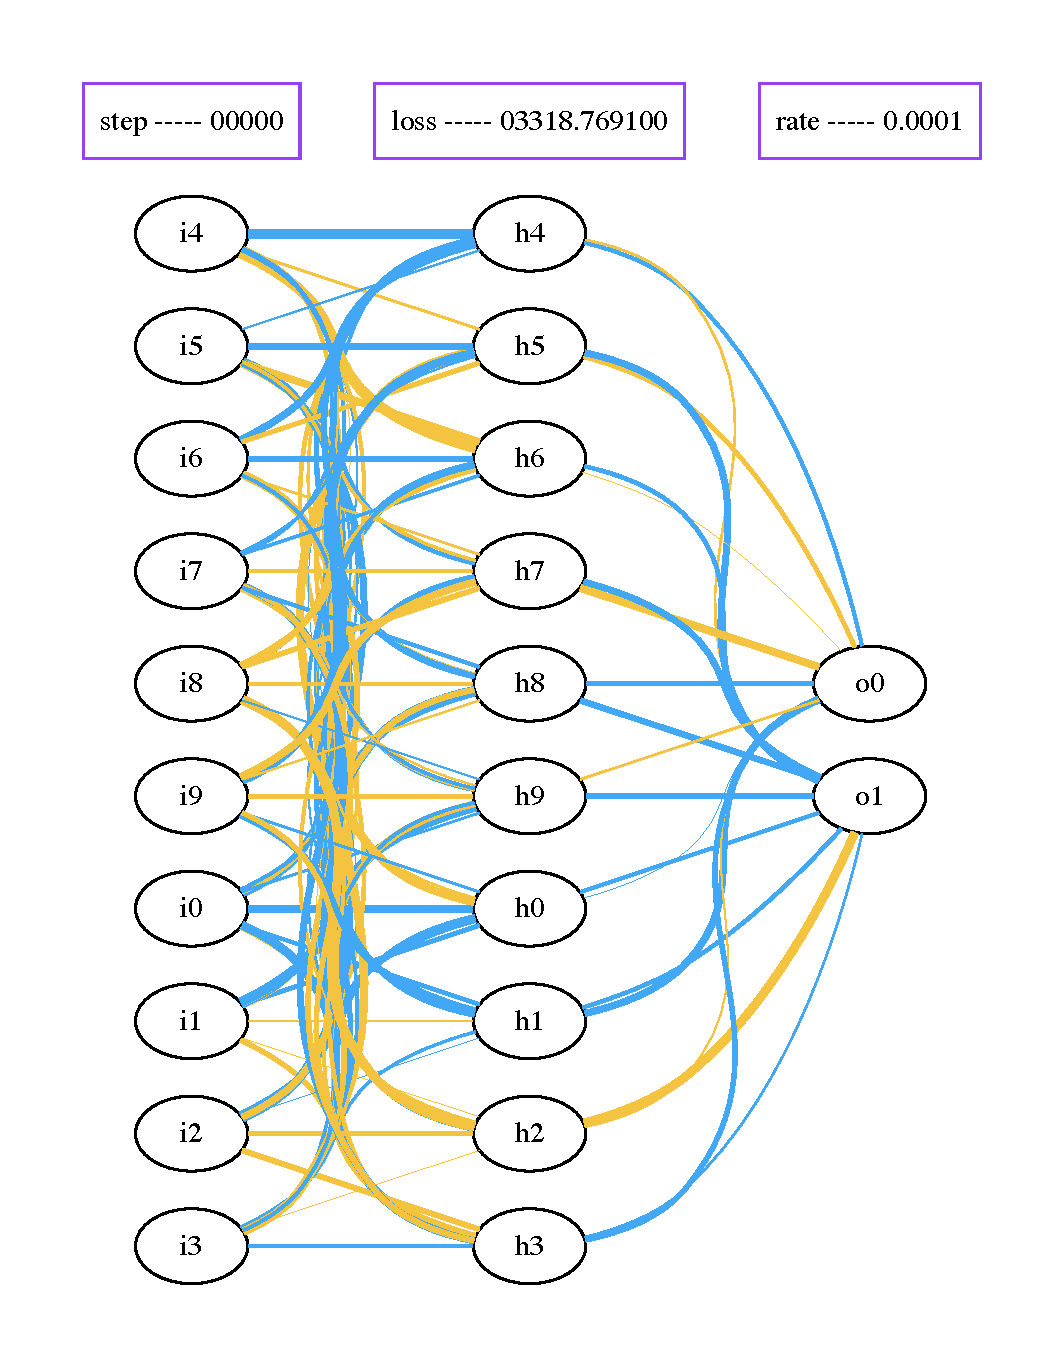
\includegraphics[width=0.1\linewidth]{net_0}
                \label{fig:name}
            \end{figure}
    \end{itemize}
\end{frame}


\begin{frame}{Matrices and networks}
    \begin{itemize}
        \item let $w=[w_{ij}]$ be the matrices of weights between neuron $i$ of
            the left layer and neuron $j$ of the middle layer.
            \begin{equation}
                b_j= \sum^{n}_{k=1}x_kw_{kj} 
            \end{equation}
        \item Finally, if we want to store the outputs for several input
            vectors $x$ ?
            \begin{figure}[htpb]
                \centering
                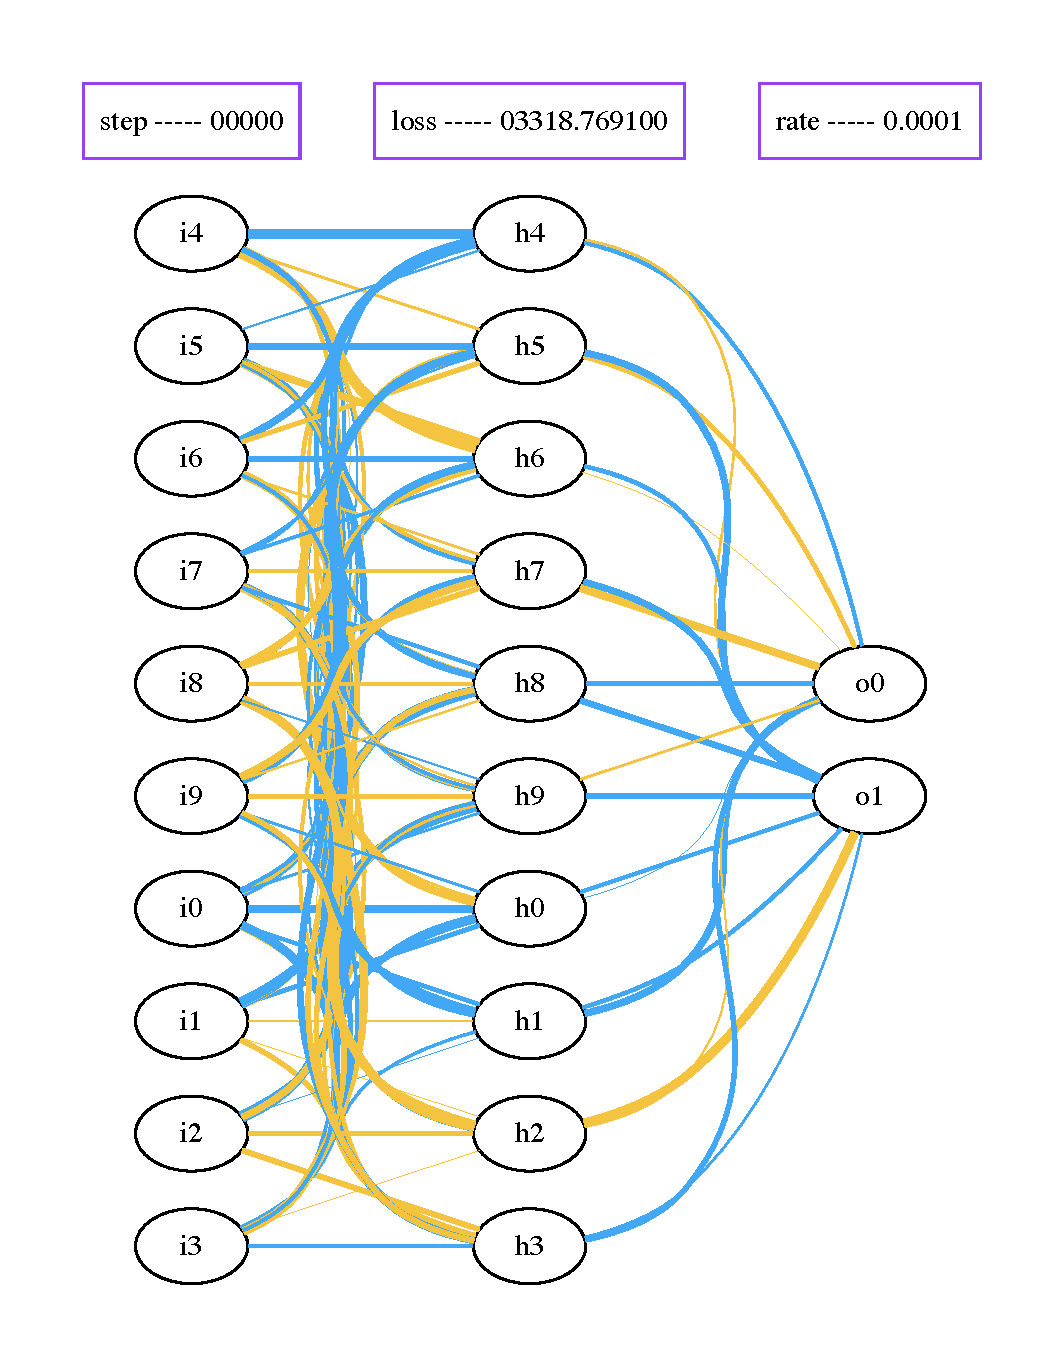
\includegraphics[width=0.1\linewidth]{net_0}
                \label{fig:name}
            \end{figure}
    \end{itemize}
\end{frame}



\begin{frame}{Matrices and networks}
    \begin{itemize}
        \item let $w=[w_{ij}]$ be the matrices of weights between neuron $i$ of
            the left layer and neuron $j$ of the middle layer.
            \begin{equation}
                b_j= \sum^{n}_{k=1}x_kw_{kj} 
            \end{equation}
        \item Finally, if we want to store the outputs for several input
            vectors $x$ ?
            \begin{itemize}
                \item use matrices  $x=[x_{ij}]$ and $b=[b_{ij}]$
                \item \begin{equation}
                        b=xw
                \end{equation}
            \end{itemize}
            \begin{figure}[htpb]
                \centering
                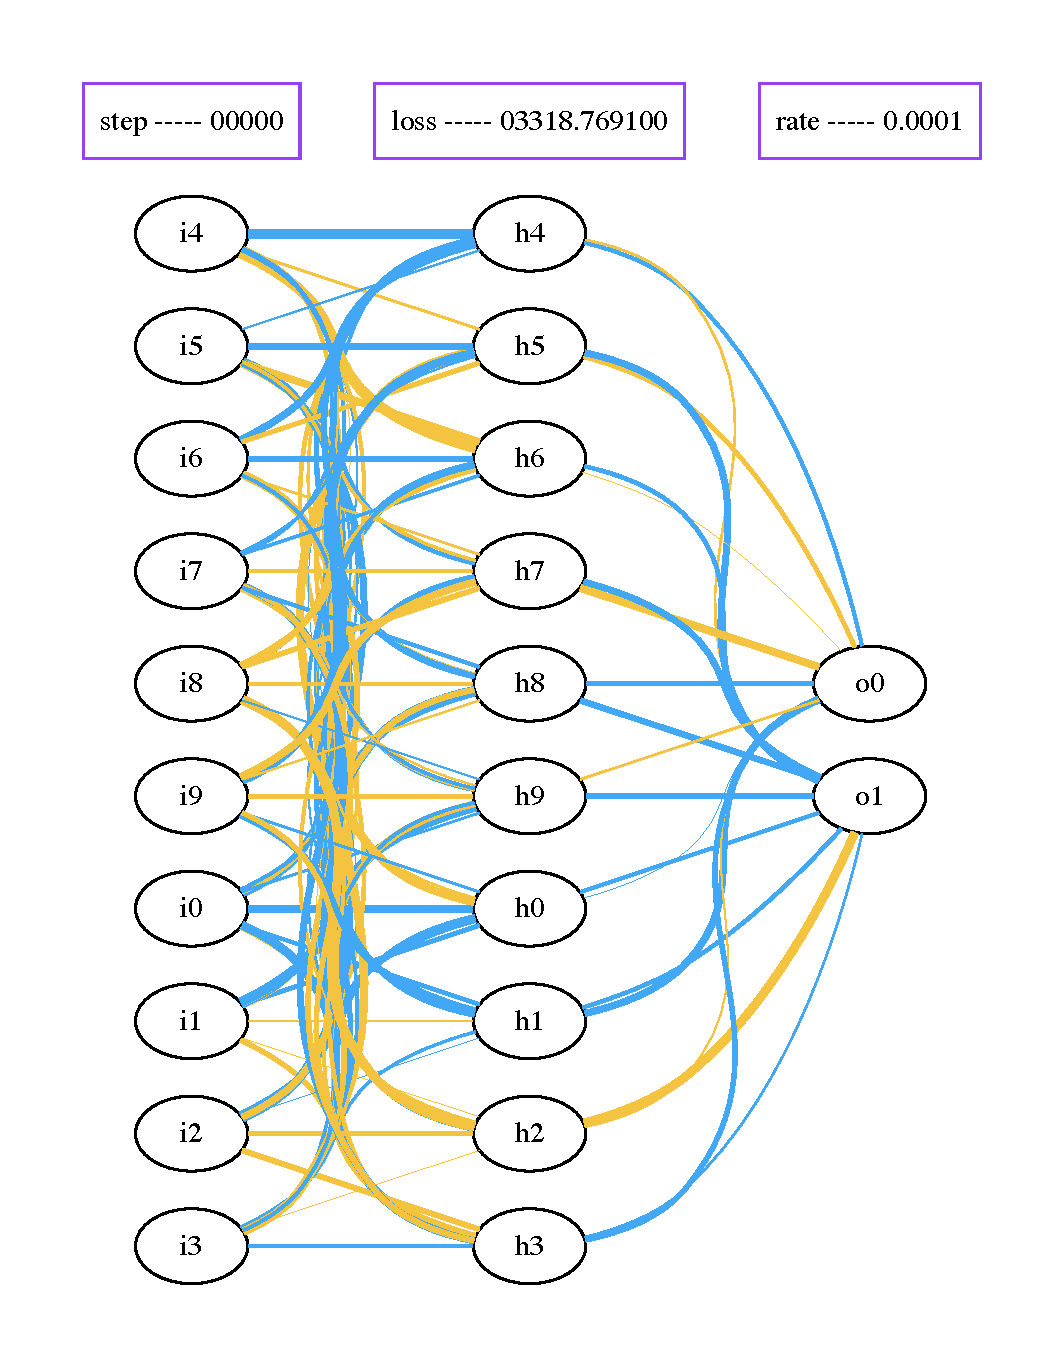
\includegraphics[width=0.1\linewidth]{net_0}
                \label{fig:name}
            \end{figure}
    \end{itemize}
\end{frame}

\begin{frame}{Layers}
    \begin{itemize}
        \item We now know how to compute the input $b$ of a layer as a function of
            the output $x$ of the previous layer  
            \begin{equation}
                b=xw
            \end{equation}
        \item Applying this rule \textbf{{and}} the non linearity $\sigma$, we
            can coompute the \textbf{{forward propagation}} of a neural
            network.
        \begin{figure}[htpb]
            \centering
            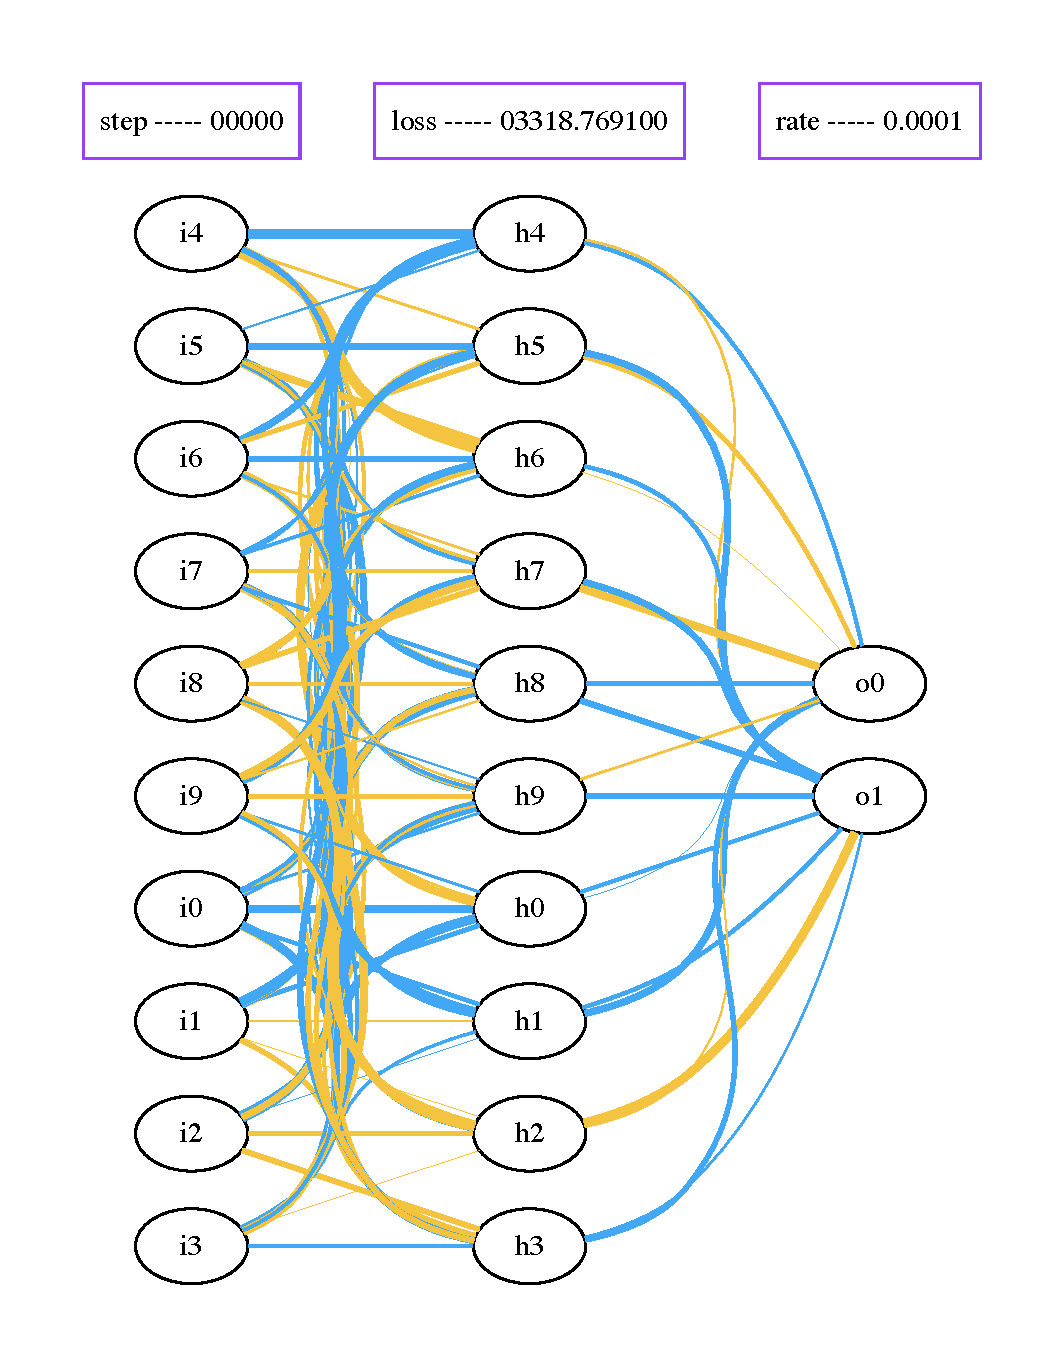
\includegraphics[width=0.3\linewidth]{net_0}
            \label{fig:net_}
        \end{figure}
    \end{itemize}
\end{frame}


\begin{frame}{Layers and forward propagation}
   \begin{itemize}
       \item We will use the \textbf{{numpy}} library to do so.
           \item In numpy, the \textbf{{.dot}} function is used to compute
               products of matrices
            \item We will use de ReLu non linearity.
   \end{itemize} 
\end{frame}

\section{Derivation, gradient descent, backpropagation}%
\label{sec:derivation_gradient_descent_backpropagation}

\begin{frame}{Cost}
    \begin{itemize}
        \item We saw how to compute the output of a neural network given an
            input
        \item But what do we want to do with the network ?
    \end{itemize}
\end{frame}

\begin{frame}{Cost}
    \begin{itemize}
        \item We saw how to compute the output of a neural network given an
            input
        \item But what do we want to do with the network ?
        \item We want to solve a given problem, for instance a
            \textbf{{supervised learning problem}} 
        \item This means being able to predict the output as a function of an
            input.
    \end{itemize}
\end{frame}

\begin{frame}{Supervised learning}
    \begin{itemize}
        \item In order to learn the prediction, we \textbf{{optimize}} our
            network with training examples
        \item What exactly do we want to optimize ?
    \end{itemize}
\end{frame}


\begin{frame}{Supervised learning}
    \begin{itemize}
        \item In order to learn the prediction, we \textbf{{optimize}} our
            network with training examples
        \item What exactly do we want to optimize ?
        \item We want to \textbf{minimize the error on the training examples.}
    \end{itemize}
\end{frame}


\begin{frame}{Supervised learning}
    \begin{itemize}
        \item In order to learn the prediction, we \textbf{{optimize}} our
            network with training examples
        \item What exactly do we want to optimize ?
        \item We want to \textbf{minimize the error on the training examples.}
        \item We will use the Squared Error
            \begin{equation}
                \sum_{\text{training samples}}\text{error}^2 
            \end{equation}
    \end{itemize}
\end{frame}


\begin{frame}{Supervised learning}
    \begin{itemize}
        \item In order to learn the prediction, we \textbf{{optimize}} our
            network with training examples
        \item What exactly do we want to optimize ?
        \item We want to \textbf{minimize the error on the training examples.}
        \item We will use the Squared Error
            \begin{equation}
              SE =   \sum_{\text{training
                samples}}(y_{\text{prediction}}-y_{\text{truth}})^2
            \end{equation}
    \end{itemize}
\end{frame}

\begin{frame}{Optimization}
    \begin{itemize}
        \item What are the \textbf{{parameters}}  of the network  ? ie : what
            we have control on and what we can change in order to minimize the
            error.
    \end{itemize}
\end{frame}


\begin{frame}{Optimization}
    \begin{itemize}
        \item What are the \textbf{{parameters}}  of the network  ? ie : what
            we have control on and what we can change in order to minimize the
            error.
        \item The \textbf{{weights}} $w_1$ and $w_2$.
        \item In our examples we will use a network with three layers : input -
            hidden - output.
            \begin{figure}[htpb]
                \centering
                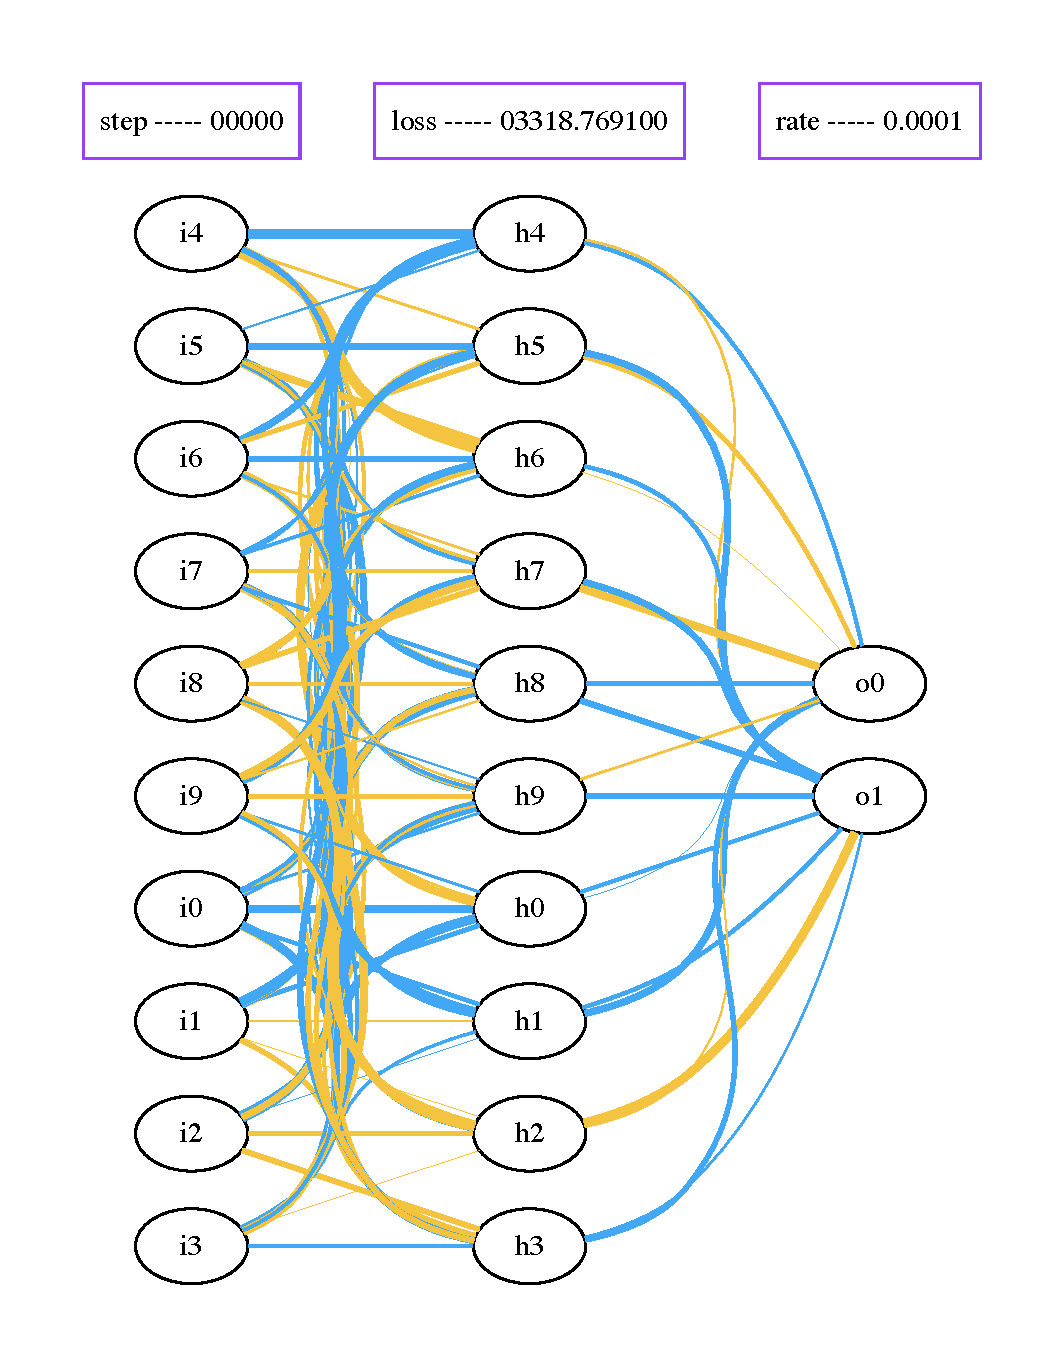
\includegraphics[width=0.3\linewidth]{net_0}
                \label{fig:name}
            \end{figure}
    \end{itemize}
\end{frame}


\begin{frame}{Optimization}
    \begin{itemize}
        \item What are the \textbf{{parameters}}  of the network  ? ie : what
            we have control on and what we can change in order to minimize the
            error.
        \item The \textbf{{weights matrices}} $w_1$ and $w_2$.
        \item In our examples we will use a network with three layers : input - hidden - output.
        \item We wee the loss as a function $L(w1,w2)$
            \begin{figure}[htpb]
                \centering
                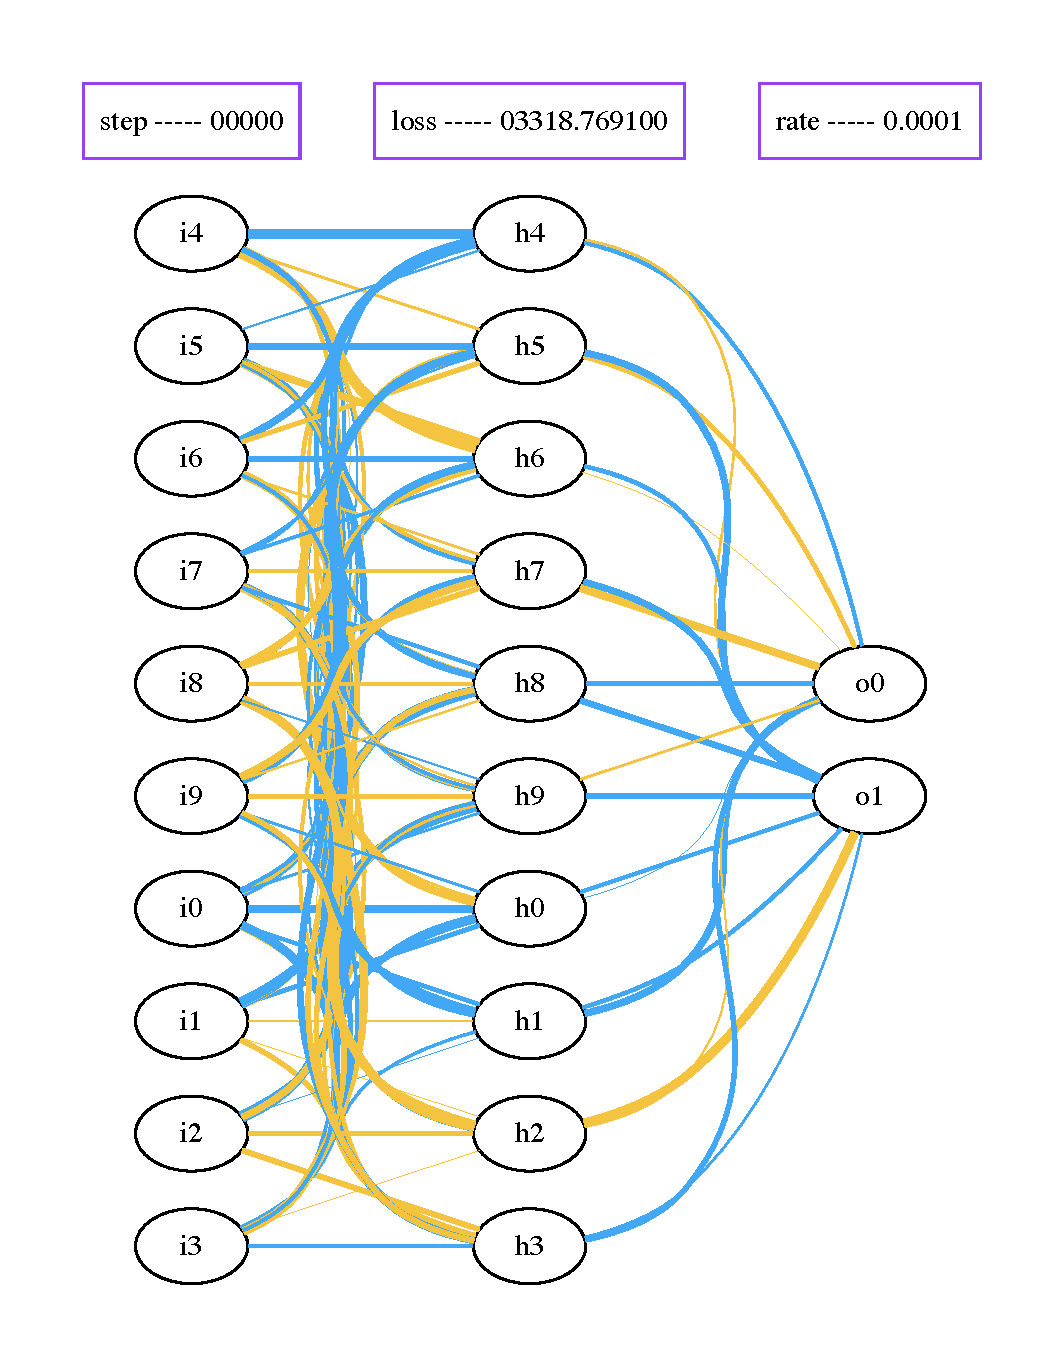
\includegraphics[width=0.3\linewidth]{net_0}
                \label{fig:name}
            \end{figure}
    \end{itemize}
\end{frame}

\begin{frame}{Gradient descent}
    \begin{itemize}
        \item In the case a function $ f : \mathbb{R}  \rightarrow
            \mathbb{R}$, we can study its variations by computing its
            derivative $f'$, \textbf{{if it exists}}
    \end{itemize}
\end{frame}

\begin{frame}{Gradient descent}
    \begin{itemize}
        \item In the case a function $ f : \mathbb{R}  \rightarrow
            \mathbb{R}$, we can study its variations by computing its
            derivative $f'$, \textbf{{if it exists}}
        \item If $f'(x)>0$, the function grows around $x$.
        \item If $f'(x)<0$, the function decreases around $x$.
        \item If $x$ is a local extremum, $f'(x)=0$

    \end{itemize}
\end{frame}


\begin{frame}{Gradient descent}
    \begin{itemize}
        \item In the case a function $ f : \mathbb{R}  \rightarrow
            \mathbb{R}$, we can study its variations by computing its
            derivative $f'$, \textbf{{if it exists}}
        \item If $f'(x)>0$, the function grows around $x$.
        \item If $f'(x)<0$, the function decreases around $x$.
        \item If $x$ is a local extremum, $f'(x)=0$
        \item Is the reciprocal true ?
    \end{itemize}
\end{frame}

\begin{frame}{Derivation}
   \begin{itemize}
       \item We can use the derivative to look for a minimum value for the
           function
        \item Example with analytic solution
   \end{itemize} 
\end{frame}

\begin{frame}{gradient}
   \begin{itemize}
       \item the \textbf{{gradient}} is similar to a derivative but in the case
           of a function with several inputs, such as our loss $l(w1,w2)$.
    \item then we store the \textbf{{partial derivative}} with respect to each
        input in a \textbf{{vector}} called the gradient. 
    \item let us compute ror instance the partial derivative with respect to $w1$ 
   \end{itemize} 
\end{frame}


\begin{frame}{gradient}
   \begin{itemize}
    \item then we store the \textbf{{partial derivative}} with respect to each
        input in a \textbf{{vector}} called the gradient. 
    \item let us compute ror instance the partial derivative with respect to $w1$ 
        \begin{equation}
            \frac{\partial L}{\partial w1}=  h^T  2(y_{\text{predicted}}-y_{{truth}})  
        \end{equation}
           (where $h$ is the output of the relu)
   \end{itemize} 
\end{frame}


\begin{frame}{Backpropagation}
   \begin{itemize}
       \item By repeating the same process we can also compute the gradient
           with respect to $w2$.
        \item This is called \textbf{{backpropagation}} 
        \item Knowing the gradient, we can \textbf{{update the network
            parameters}} 
   \end{itemize} 
\end{frame}

\begin{frame}{Application to our neural network}
   \begin{itemize}
       \item We will apply this to do some supervised learning over two
           datasets:
           \begin{itemize}
               \item A random dataset
                   \item A structured dataset
           \end{itemize}
   \end{itemize} 
\end{frame}

\begin{frame}{Libs}
    \begin{itemize}
        \item We will need \textbf{{numpy}} 
            \item \textbf{{pygraphviz}} 
            \item optionally \textbf{{pytorch}}  (less important for us today)
                    \item It will most probably work better with python3.6
    \end{itemize}
\end{frame}

\section{Visualizing some neural nets}%
\label{sec:visualizing_some_neural_nets}

\begin{frame}{Exercise 1}
   \begin{itemize}
       \item \textbf{{cd neural\textunderscore net}} 
        \item Use \textbf{{learn\textunderscore random \textunderscore data}}
            to learn to predict some output as a function of some input
        \item You will need to tune some hyperparameters.
   \end{itemize} 
\end{frame}


\begin{frame}{Exercise 2}
   \begin{itemize}
        \item Now make it find a local minimum that is not global
   \end{itemize} 
\end{frame}



\begin{frame}{Exercise 3}
   \begin{itemize}
       \item Now make it explode (diverge)
   \end{itemize} 
\end{frame}

\begin{frame}{Exercise 4}
   \begin{itemize}
       \item  Uncomment the lines calling \textbf{{show\textunderscore net}} so
           plot the evolution of the network
        \item You might need to use a smaller network otherwise it will be too
            long.
            \begin{figure}[htpb]
                \centering
                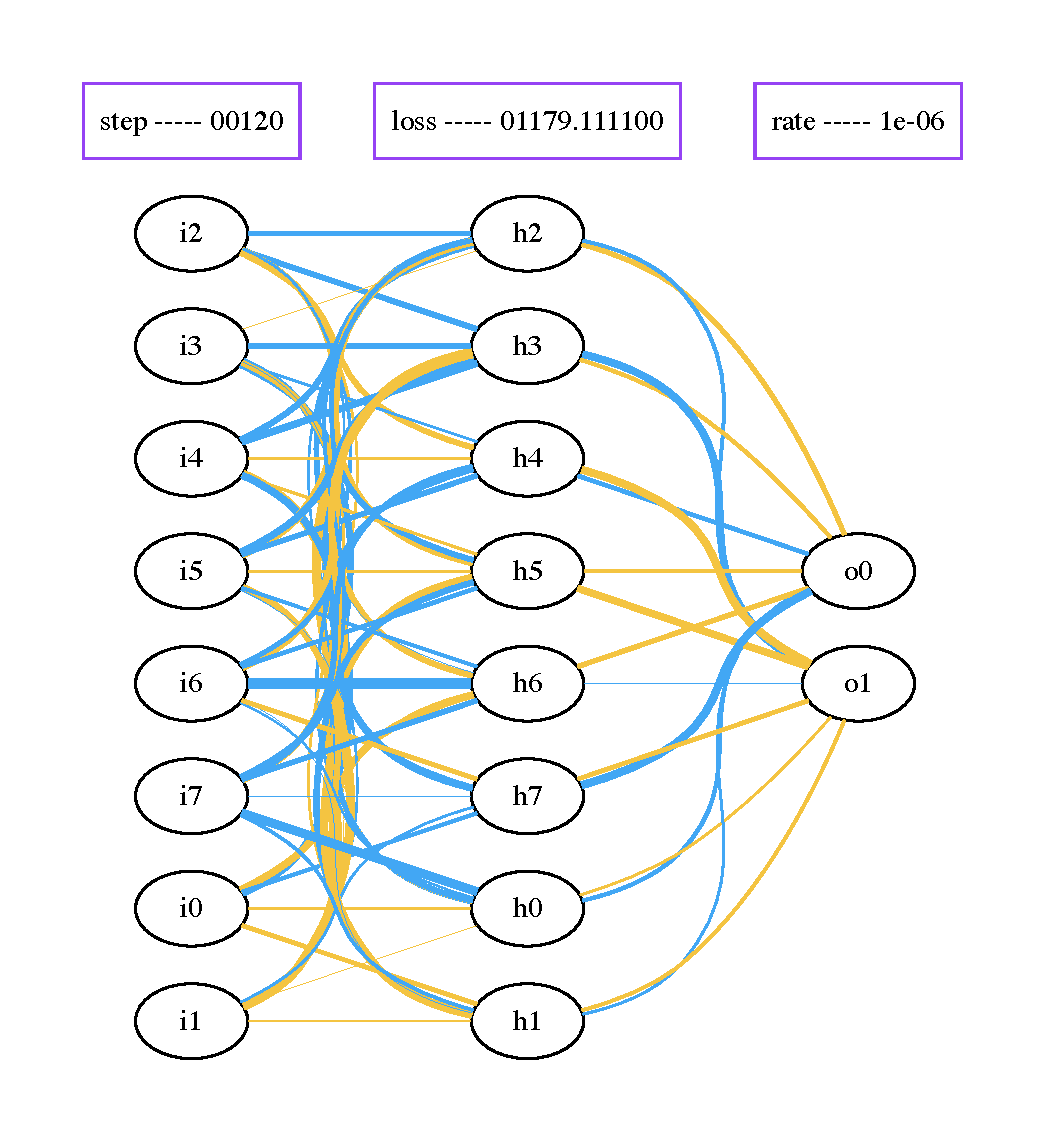
\includegraphics[width=0.5\linewidth]{net_120}
                \caption{}
                \label{fig:}
            \end{figure}
   \end{itemize} 
\end{frame}

\begin{frame}{Exercise 5}
    \begin{itemize}
        \item Does this make sense ?
            \item Can we generalize what we learned ?
    \end{itemize}
\end{frame}

\begin{frame}{exercise 5}
    \begin{itemize}
        \item does this make sense ?
            \item can we generalize what we learned ?
                \item since the data are random, and not correlated, we are not
                    learning any structure in them
    \end{itemize}
\end{frame}


\begin{frame}{exercise 5}
    \begin{itemize}
        \item does this make sense ?
            \item can we generalize what we learned ?
                \item since the data are rando, and not correlated, we are not
                    learning any structure in them
                \item What is the test error ? (use the relevant function)
    \end{itemize}
\end{frame}

\begin{frame}{Exercise 6}
    \begin{itemize}
        \item We will now use structured data
            \item They are artificially generated in
                \textbf{{create\textunderscore structured\textunderscore data}} by a function, with a noise that you can choose
                \item You can tune the standard deviation of the noise
            \item Use \textbf{{create\textunderscore structured\textunderscore
                data}} and \textbf{{learn\textunderscore structured\textunderscore data}} to generate a dataset and learn it in a
                supervised way
    \end{itemize}
\end{frame}


\begin{frame}{Exercise 7}
    \begin{itemize}
    \item Make it find a local minimum
    \end{itemize}
\end{frame}

\begin{frame}{Exercise 8}
    \begin{itemize}
    \item Make it explode
    \end{itemize}
\end{frame}


\begin{frame}{Exercise 9}
    \begin{itemize}
    \item Uncomment the relevant stuff to visualize the evolution of the
        network with graphviz
    \item You wan choose the number of hidden layers
    \end{itemize}
\end{frame}

\begin{frame}{exercise 10}
    \begin{itemize}
        \item how does the test error behave ?
    \end{itemize}
\end{frame}
\begin{frame}{exercise 10}
    \begin{itemize}
        \item how does the test error behave ?
            \item Now it makes more sense since we worked on data with
                structure
    \end{itemize}
\end{frame}

\begin{frame}{With libs}
    \begin{itemize}
        \item We did things manually with numpy but when the networks are large
            or when we need to automate the seach for good parameters, it is
            more convenient to work with libraries such as :
            \begin{itemize}
                \item pytorch
                    \item tensorflow
                        \item keras
            \end{itemize}
    \end{itemize}
\end{frame}

\section{Other techniques}%
\label{sec:other_techniques}

\begin{frame}{Many techniques}
    \begin{itemize}
        \item There are lots of variations around neural nets
            \begin{itemize}
                \item in the number of neurons per layer
                    \item type of data processed
                    \item relationship between weights (shared weights)
                        \item number of hidden layers
                        \item recurrent neural networks RNN
                            \item convolutional neural networks CNN
            \end{itemize}
    \end{itemize}
\end{frame}

\begin{frame}{Stochastic gradient}
    \begin{itemize}
        \item Another method to compute the gradient
    \end{itemize}
\end{frame}


\begin{frame}{Other cost functions}
   \begin{itemize}
       \item  Until now we used the squared error cost function
           \item The slowdown problem
               \item The Cross entropy is another possible cost function used
                   for classification
   \end{itemize} 
\end{frame}

\end{document} 
